\subsection {Sprint 4}

Após todos os ajustes já realizados no \textit{frontend} para se adequar aos padrões visuais expostos no protótipo feito pelo time de \textit{design} do Lab Livre, a quarta \textit{sprint} foi caracaterizada por um único requisito: ter tabelas no texto. No respositório oficial do Trix há uma \textit{issue}, já fechada, onde usuários questionam se há planos de adicionar o suporte a tabelas; até a data deste trabalho não houve indícios de que mantenedores do projeto irão atuar nessa demanda. A \textit{issue} mencionada pode ser acessada em \url{https://github.com/basecamp/trix/issues/539}.

\subsubsection {Requisito 1 da Sprint 4}

Dada a limitação do Trix em relação ao uso de tabelas, anteriormente foi acordado com o time de produto do Lab Livre que estas seriam inseridas no texto no formato de imagens. Entretanto, em reuniões de \textit{feedback} com os \textit{stakeholders}, viu-se que era impraticável em termos de experiência do usuário e usabilidade proceder dessa maneira.
Foram feitas reuniões de descorberta com o time responsável pela plataforma Participa+ Brasil, onde existe funcionalidade semelhante ao texto participativo, e que existe o suporte a tabelas. Como saída dessa reunião foram sugeridos alguns editores de texto, dentre eles: Jodit, CKEditor 5 e o TinyMCE. No Participa+ Brasil é utilizado o editor Jodit. Com base na premissa de que alguns usuários poderiam migrar do Participa+ Brasil para o Brasil Participativo, o Jodit foi escolhido como potencial escolha.

Para garantir que haveria compatibilidade com a ferramenta de textos do Brasil Participativo, foi realizado um teste localmente, trocando o Trix pelo Jodit na página de inserção de conteúdo para criação de texto participativo.
O teste foi realizado inserindo na própria \textit{view} da página \textit{links} para o JavaScript e o CSS do Jodit, conforme descrito na própria documentação do editor. Para validar a viabilidade de uso do editor, foram feitas várias provas inserindo tabelas, imagens e textos formatados através do comando de copiar e colar, todos os textos vindo do Google Docs, Microsoft Word e LibreOffice Writer. Foram manualmente persistidos alguns parágrafos que continham tabelas, e posteriormente exibidos com sucesso na tela de visualização do texto participativo.

Com o sucesso desses testes, o desenvolvimento finalmente seguiria com foco total na implantação do Jodit no Brasil Participativo. Como próximo passo, era preciso, da mesma forma como foi feito para o Trix, achar formas de persistir as imagens inseridas no editor no \texttt{storage}. O Jodit possui a opção \texttt{uploader.insertImageAsBase64}, que guarda o conteúdo da imagem no formato de Data URL na própria estrutura do HTML.
Data URL é uma maneira de embutir o conteúdo de arquivo de forma \textit{inline} em documentos \cite{data-urls-mdn}. O atributo \texttt{src} de \textit{tags} \texttt{<img>} é preenchido com o próprio conteúdo da imagem codificado em Base64, ao invés de ter um \textit{link} para onde esta estaria guardada.

Dessa maneira, ao invés de tentar guardar a imagem no \texttt{storage} logo que for inserida no texto, pode-se guardá-la apenas quando o usuário submeter o texto para criação.
Na forma como era feita com o Trix, caso o usuário arrastasse uma imagem para o editor e depois a removesse antes mesmo de submeter o texto, esta ficaria sem qualquer uso, e mesmo assim continuaria persistida no \texttt{storage}. Com o uso de Data URLs, é possível evitar esses casos e ter maior controle do ciclo de vida das imagens.

Sendo assim, o próximo passo seria, então, fazer o \textit{parsing} do \textit{input} HTML e realizar a divisão dos parágrafos. Diferentemente do Trix que por padrão inseria novos paragrafos envoltos de \textit{tags} \texttt{<div>}, da forma como foi configurado, no Jodit os parágrafos são envoltos de \textit{tags} \texttt{<p>}, e a cada quebra de linha uma nova \textit{tag} \texttt{<p>} é criada para servir de container para o texto.
O único problema é a formatação de alguns textos quando copiados do Google Docs e do Microsft Word. Alguns utilizam \textit{tags} \texttt{<p>} para servir de container para \textit{tags} \texttt{<img>}, além de em alguns momentos o texto de vários parágrafos estar envolto de uma única \textit{tag} \texttt{<strong>}. Esse comportamento foi classificado neste trabalho como "\textit{tags} modificadoras de texto sendo utilizadas como \texttt{<div>}", e guiou o desenvolvimento do \textit{parser} para suportar a migração para o Jodit.

A versão final do \textit{parser} de textos participativos executa três passos:

\begin{enumerate}
	\item Substituir sequência de caracteres de espaço em branco ou não imprimíveis por um único espaço no \textit{input} HTML ainda em formato \texttt{string};
	\item Realizar a transformação para a estrutura do Nokogiri;
	\item Separar parágrafos removendo aqueles que estivem em branco.
\end{enumerate}

A figura \ref{fig:jodit-parser-final} demonstra o código fonte da etapa de \textit{parsing} do \textit{input}.

\begin{figure}[htbp]
  \centering
  \caption{Código fonte da função que realiza o \textit{parsing} do HTML vindo do Jodit}
  \label{fig:jodit-parser-final}
  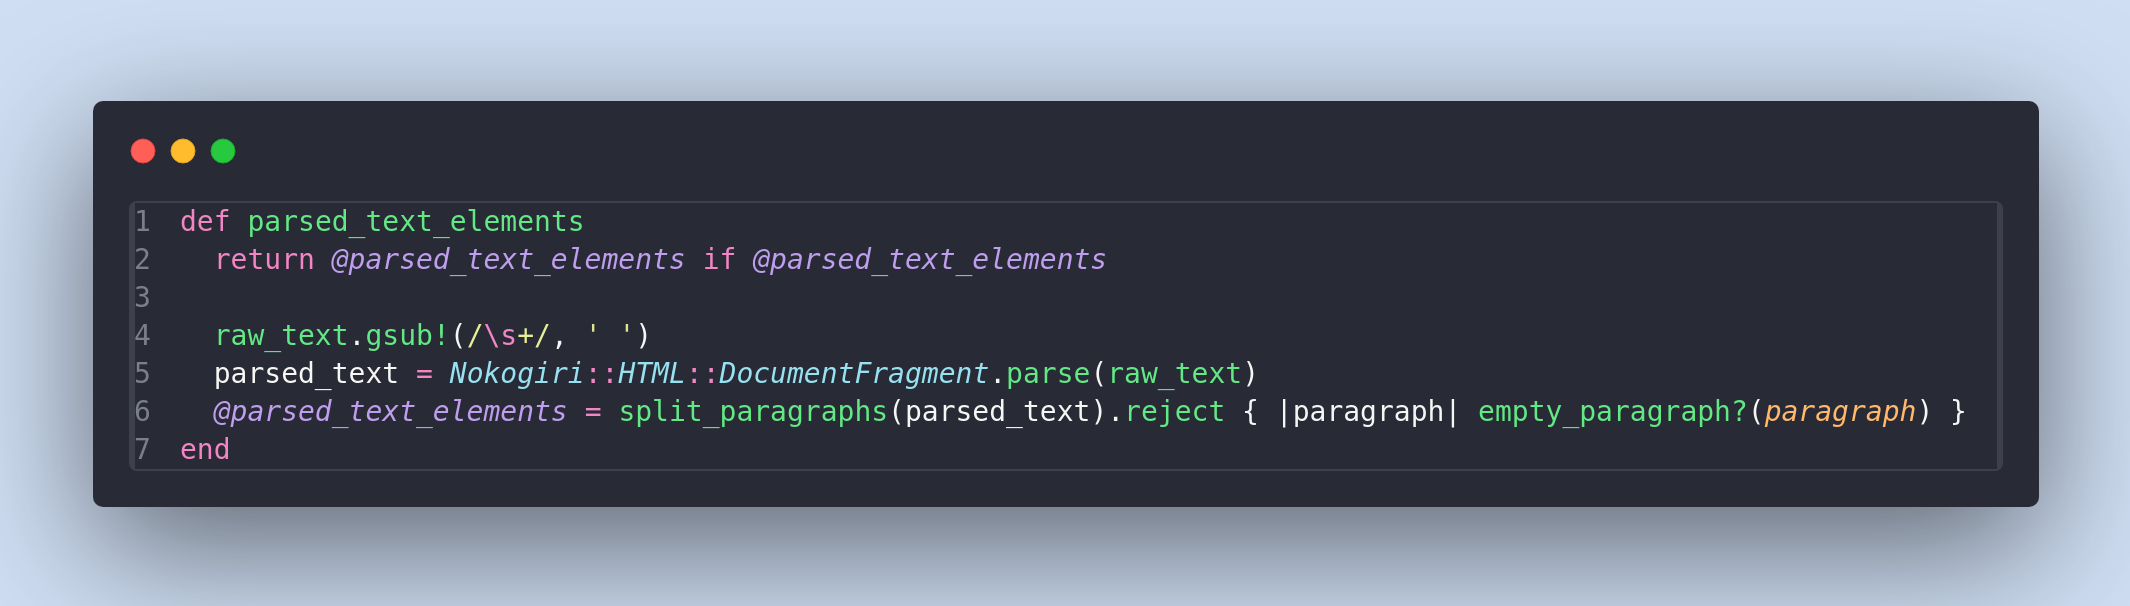
\includegraphics[width=\textwidth]{figuras/jodit-parser-final.png}
  \fonte{Próprio autor}
\end{figure}

O método \texttt{split\_paragraphs} é um método também criado a mão para satisfazer os casos de bordas classificados como "\textit{tags} modificadoras de texto sendo utilizadas como \texttt{<div>}". Para resolver esse problema, foi utilizada uma estratégia recursiva para percorrer a árvore de nós do Nokogiri e determinar quais nós pertencem ao mesmo parágrafo ou não.

A verificação começa no nó raiz, que é o próprio \texttt{DocumentFragment}. Se o nó que está sendo avaliado nesse momento for uma \texttt{<div>} ou o \texttt{DocumentFragment}, recursivamente chama a verificação para todos os seus nós filhos retornados pelo método \texttt{children}, pegando o resultado e compilando em um \texttt{Array} achatado, isto é, um \texttt{Array} que não possui elementos do tipo \texttt{Array} dentro de si. A mesma coisa também é feita caso o nó seja um modificador de texto sendo usado como \texttt{<div>}. Caso contrário, é retornado um \texttt{Array} envolvendo o próprio nó apenas. A ideia central por trás desse algoritmo é a de eliminar elementos que sejam uma \texttt{<div>} ou que ajam como uma \texttt{<div>}, e escolher ramos da árvore para serem parágrafos. O código fonte dessa verificação pode ser visto na Figura \ref{fig:split-paragraphs-jodit}.

\begin{figure}[htbp]
  \centering
  \caption{Código fonte do método que realiza a divisão de parágrafos do Jodit}
  \label{fig:split-paragraphs-jodit}
  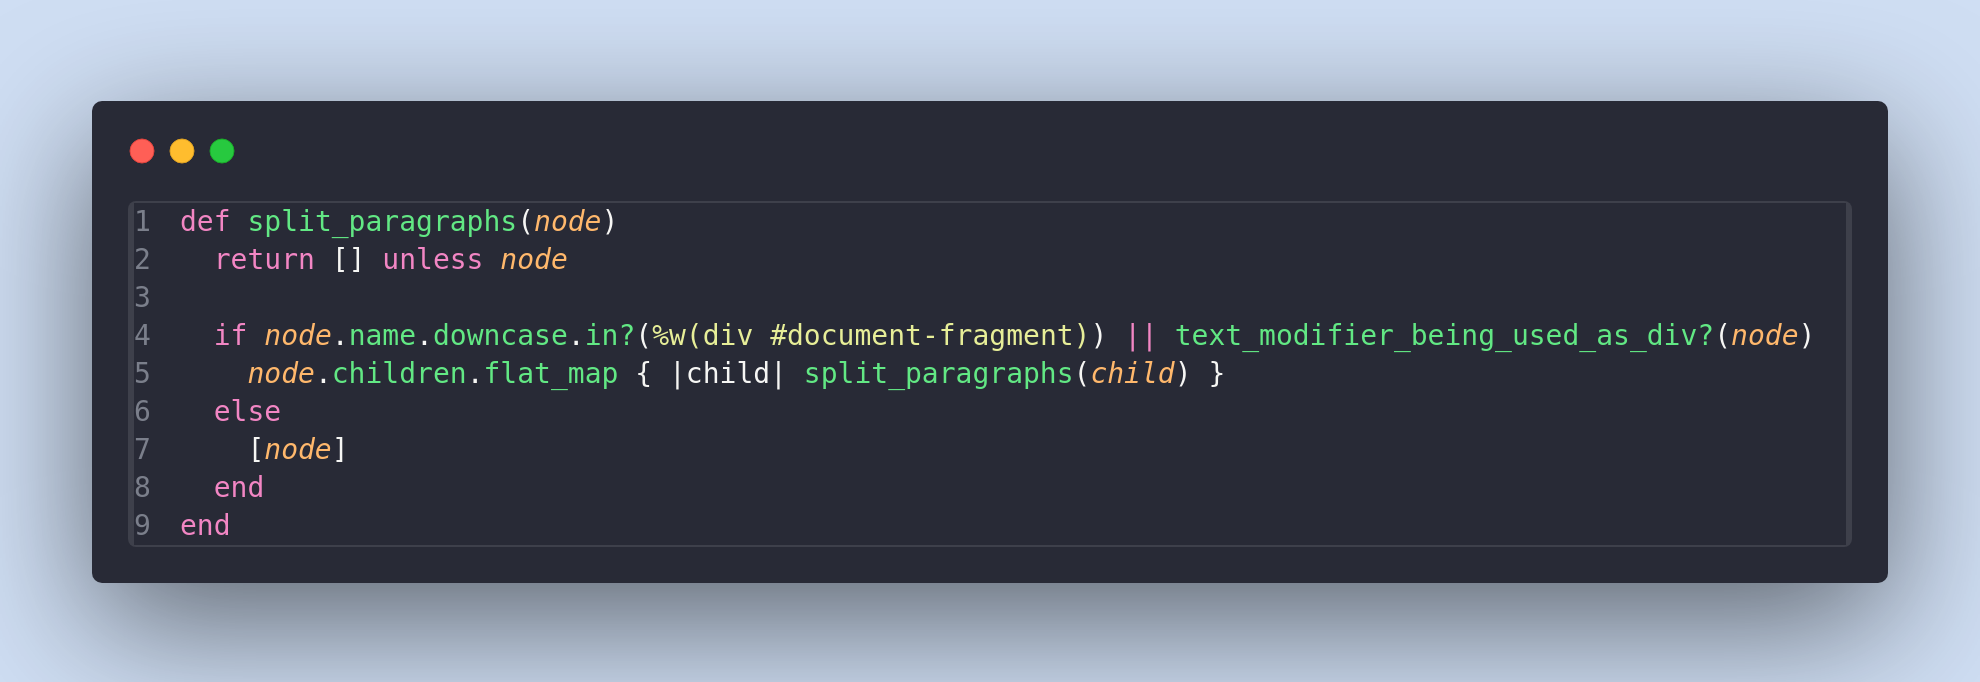
\includegraphics[width=\textwidth]{figuras/split-paragraphs-jodit.png}
  \fonte{Próprio autor}
\end{figure}

O algoritmo para definir se um determinado nó está sendo usado como \texttt{<div>} também é de caráter recursivo. A análise começa no primeiro nó passado como parâmetro. Primeiro se verifica se o nó é uma \textit{tag} modificadora de texto, se não for, o algoritmo para e a resposta é falso. Caso contrário, o algoritmo segue em frente e verifica se o nó atual possui filhos, se não tiver, ele para e a resposta é falso. Caso contrário, o algoritmo segue em frente e passa a avaliar todos os filhos diretos do nó que está sendo avaliado. Recursivamente o algoritmo irá avaliar para cada filho se este é uma \textit{tag} modificadora sendo usada como \texttt{<div>}. Se ao menos um de seus filhos for uma \textit{tag} modificadora sendo usada como \texttt{<div>}, o próprio nó também será considerado, e o algoritmo retorna verdadeiro. Na Tabela \ref{tab:tags-html-modificadoras-de-texto} está a relação de \textit{tags} que são consideradas modificadoras de texto. Vale notar que a \textit{tag} \texttt{<img>} está entre elas, pois uma imagem, nesse contexto, tem o valor semântico que um texto puro dentro de um parágrafo. Isto é, uma imagem não é fator determinante para dividir um parágrafo. O código fonte dessa verificação pode ser visto na Figura \ref{fig:text-modifier-beign-used-as-div-jodit}.

\begin{table}[h]
	\centering
	\caption{\textit{Tags} HTML modificadoras de texto}
	\label{tab:tags-html-modificadoras-de-texto}
	\begin{tabular}{c}
    \toprule
		p \\
		title \\
		span \\
		br \\
		text \\
		strong \\
		b \\
		em \\
		i \\
		u \\
		s \\
		del \\
		mark \\
		small \\
		sup \\
		code \\
		pre \\
		img \\
		a \\
		\bottomrule
	\end{tabular}
\end{table}

\begin{figure}[htbp]
  \centering
  \caption{Código fonte do método que verifica se modificador de texto está sendo usado como \texttt{<div>}}
  \label{fig:text-modifier-beign-used-as-div-jodit}
  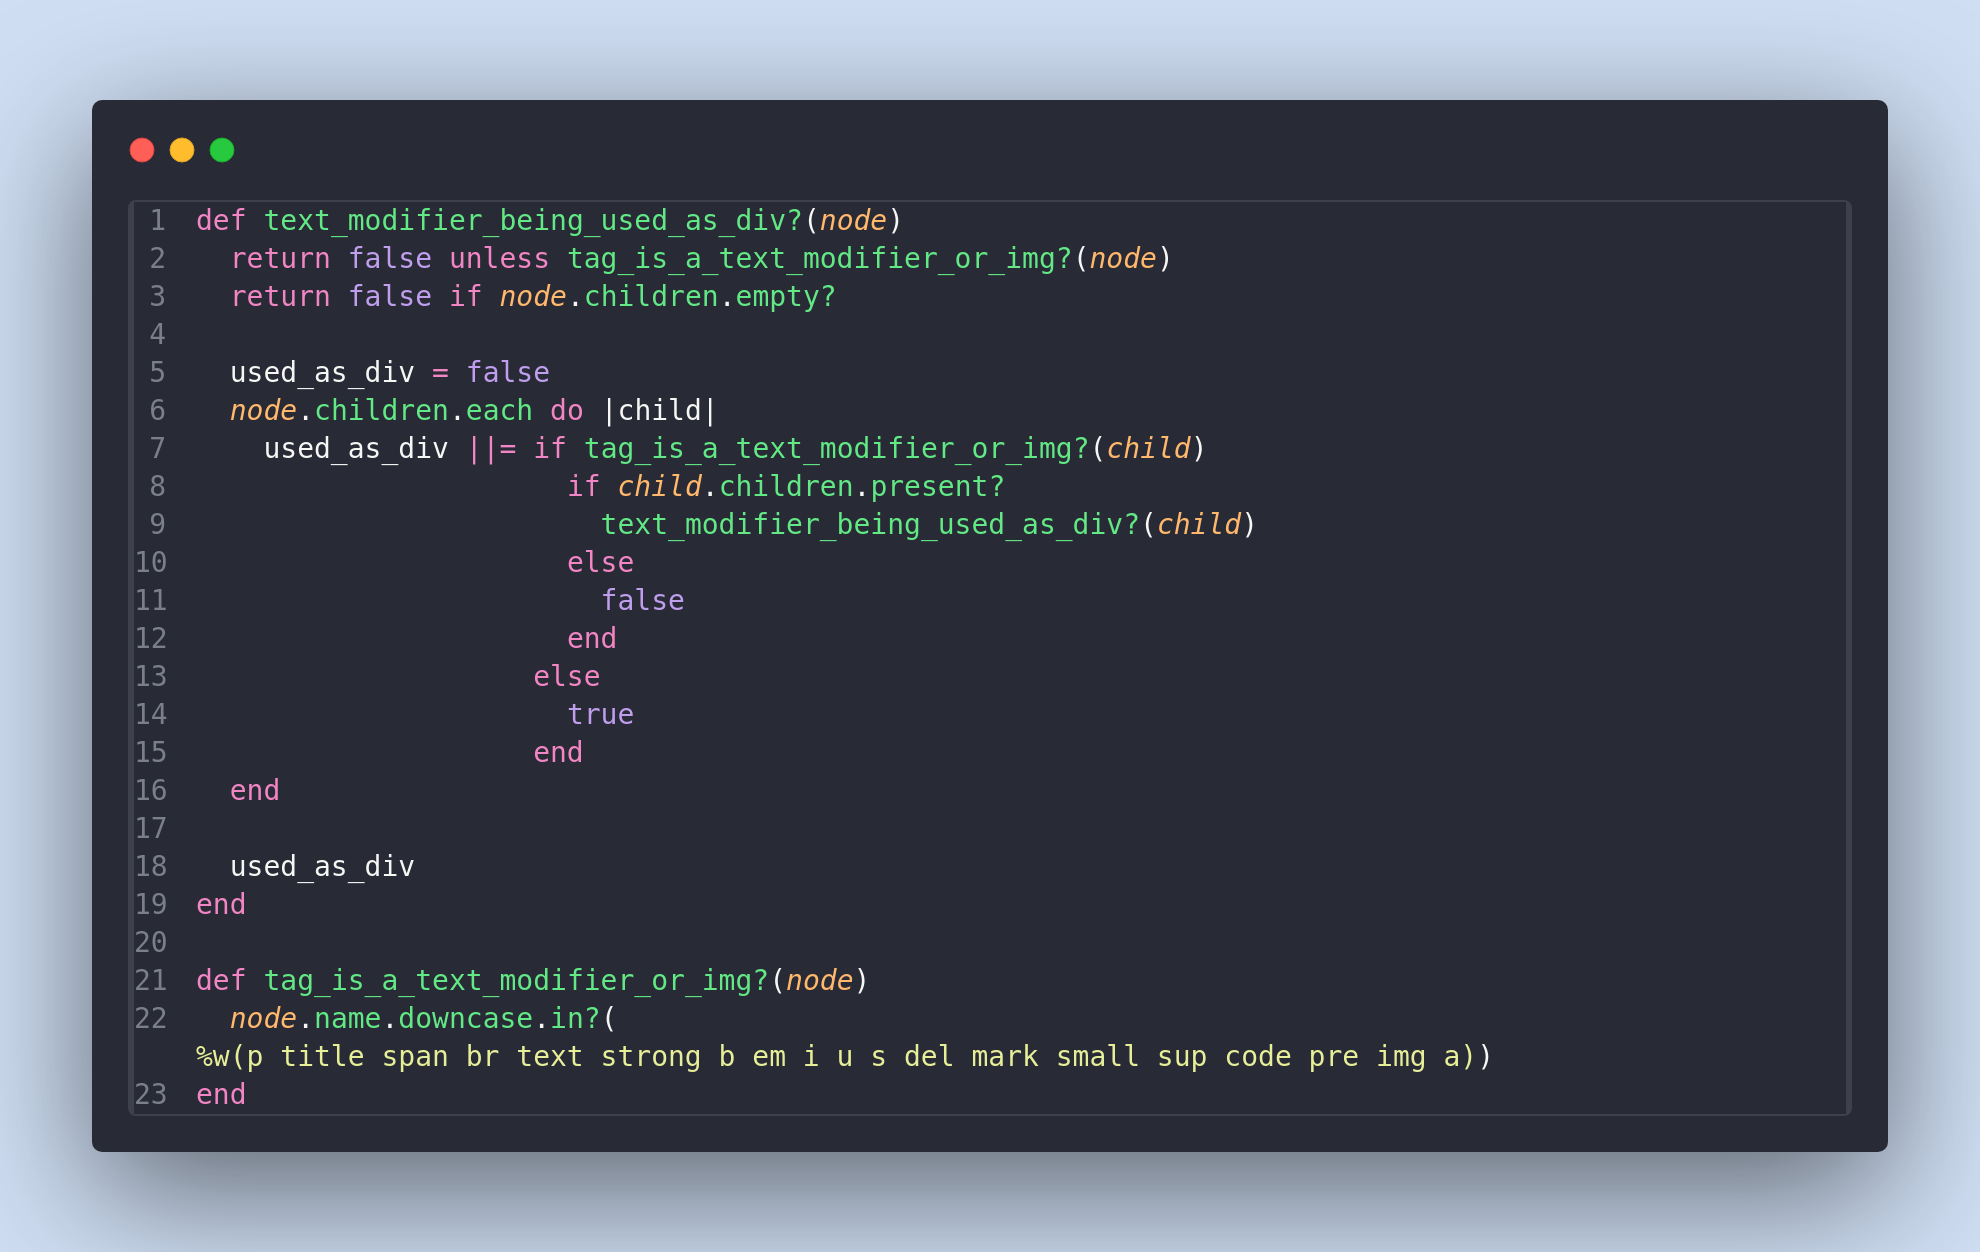
\includegraphics[width=\textwidth]{figuras/text-modifier-being-used-as-div-jodit.png}
  \fonte{Próprio autor}
\end{figure}

O \textit{Merge Request} com as alterações dessa \textit{sprint} pode ser encontrado em \url{https://gitlab.com/lappis-unb/decidimbr/decidim-govbr/-/merge_requests/641}